\section{Experiments}
\subsection{Preprocessing}
The dataset is quite big to handle contain 3 file: \\
    - Books.csv: 271379 records \\
    - Users.csv: 276271 records \\ 
    - \textbf{Ratings.csv: 1149781 records} \\
    
Therefore, we are using the map-reduce technique to split the data in order to fit the computer memory.

The map reduce is using to group and count all pair of books bought by at least 2 users and running on file Ratings.csv. 

Map reduce first phase: 
    % \begin{figure}[H]
    %     \centering
    %     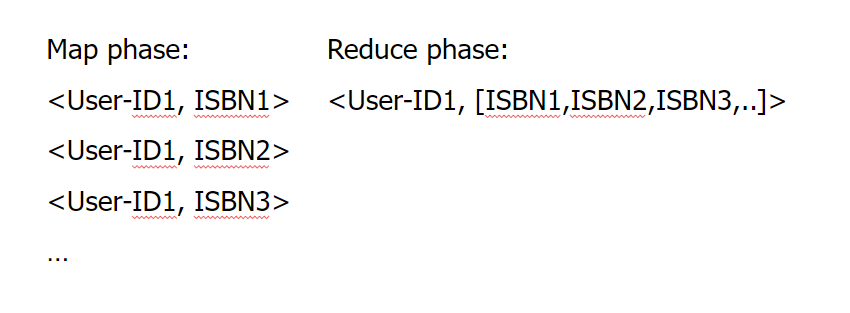
\includegraphics[width=\textwidth]{image/mapreduce 1.png}
    %     \caption{Map reduce first phase find all books were bought by single users}
    % \end{figure}

    \begin{table}[H]
        \centering
        \begin{tabular}{|l|l|}
            \hline
             \textbf{Map phase}       &  \textbf{Reduce phase}\\ \hline
             <User-ID1, ISBN1> & <User-ID1, [ISBN1, ISBN2, ISBN3, ...]> \\
             <User-ID1, ISBN2> & \\
             <User-ID1, ISBN3> & \\ \hline
        \end{tabular}
        \caption{Map reduce first phase find all books were bought by single users}
        \label{tab:my_label}
    \end{table}

Map second phase: 
    % \begin{figure}[H]
    %     \centering
    %     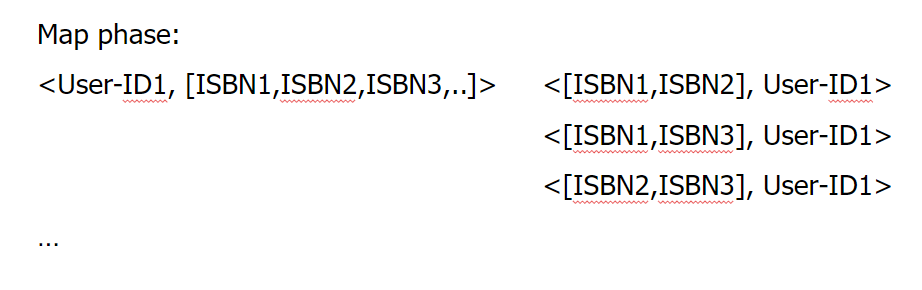
\includegraphics[width=\textwidth]{image/mapreduce 2.png}
    %     \caption{Map phase to find all books pair of book bought by users}
    % \end{figure}

    \begin{table}[H]
        \centering
        \begin{tabular}{|l|l|}
            \hline
             \textbf{Map phase}      &  \\ \hline
             <User-ID1, [ISBN1, ISBN2, ISBN3, ...]> & <[ISBN1, ISBN2], User-ID1> \\
                               & <[ISBN1, ISBN3], User-ID1>\\
                               & <[ISBN2, ISBN3], User-ID1>\\ \hline
        \end{tabular}
        \caption{Map phase to find all books pair of book bought by users}
        \label{tab:my_label}
    \end{table}

Reduce second phase: 
    % \begin{figure}[H]
    %     \centering
    %     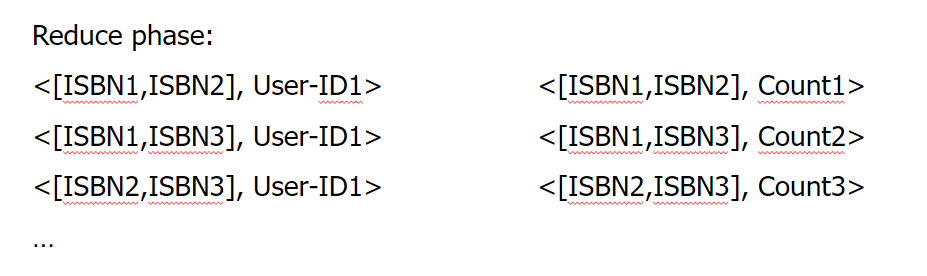
\includegraphics[width=\textwidth]{image/mapreduce 3.png}
    %     \caption{Reduce phase to find all books pair of books and number of users bought it}
    % \end{figure}

    \begin{table}[H]
        \centering
        \begin{tabular}{|l|l|}
            \hline
            \textbf{Reduce phase} &  \\ \hline
             <[ISBN1, ISBN2], User-ID1> & <[ISBN1, ISBN2], Count1> \\
             <[ISBN1, ISBN3], User-ID1> & <[ISBN1, ISBN3], Count2> \\
             <[ISBN2, ISBN3], User-ID1> & <[ISBN2, ISBN3], Count3> \\ \hline
        \end{tabular}
        \caption{Reduce phase to find all books pair of books and number of users bought it}
        \label{tab:my_label}
    \end{table}

% \subsection{Evaluation}


\subsection{Build application}

We built a web application to demonstrate the process of recommendation in book store. Web are built with VueJS as a Frontend and Flask as a framework by Python language programming. Backend is in charge of query similar books and return it to Frontend via Restful api.

\begin{figure}[H]
    \centering
    
\includegraphics[width=0.7\textwidth]{image/technology.png}
    \caption{Technologies used}
\end{figure}

\subsubsection{Build Backend}
\textbf{Flask introduction:} Flask is a micro web framework written in Python. It is classified as a microframework because it does not require particular tools or libraries. It has no database abstraction layer, form validation, or any other components where pre-existing third-party libraries provide common functions.

\textbf{All required libraries:} \\
Create file \textit{requirements.txt}:
\begin{lstlisting}
Flask==2.2.3
Flask-Cors==3.0.10
pandas==2.0.0
networkx==2.8.8
\end{lstlisting}

\textbf{Install all libraries via command:}
\begin{lstlisting}
pip install -r requirements.txt
\end{lstlisting}

\textbf{Run backend locally on port 5000}
\begin{lstlisting}
python main.py
\end{lstlisting}
\subsubsection{Build Frontend}
\textbf{VueJS introduction:} Vue.js is an open-source model–view–viewmodel front end JavaScript framework for building user interfaces and single-page applications. It was created by Evan You, and is maintained by him and the rest of the active core team members

\subsubsubsection{Components}

Include 3 pages
\begin{enumerate}
    \item Homepage: Some categories, and popular items among users
    \begin{figure}[H]
            \centering
            
\includegraphics[width=\textwidth]{image/homepage.jpg}
            \caption{Homepage}
        \end{figure}

    \begin{figure}[H]
            \centering
            
\includegraphics[width=\textwidth]{image/homepage2.jpg}
            \caption{Book category in homepage}
        \end{figure}

    \item Book category page: All books in E-Commerce using pagination.
    \begin{figure}[H]
            \centering
            
\includegraphics[width=\textwidth]{image/book category.jpg}
            \caption{Book category page}
        \end{figure}

    \item Book detail page: Detail of a book and all similar book using Louvain, Leiden, Girvan Newman.
    \begin{figure}[H]
            \centering
            
\includegraphics[width=\textwidth]{image/book-detail.jpg}
            \caption{Book detail page}
        \end{figure}

    \begin{figure}[H]
            \centering
            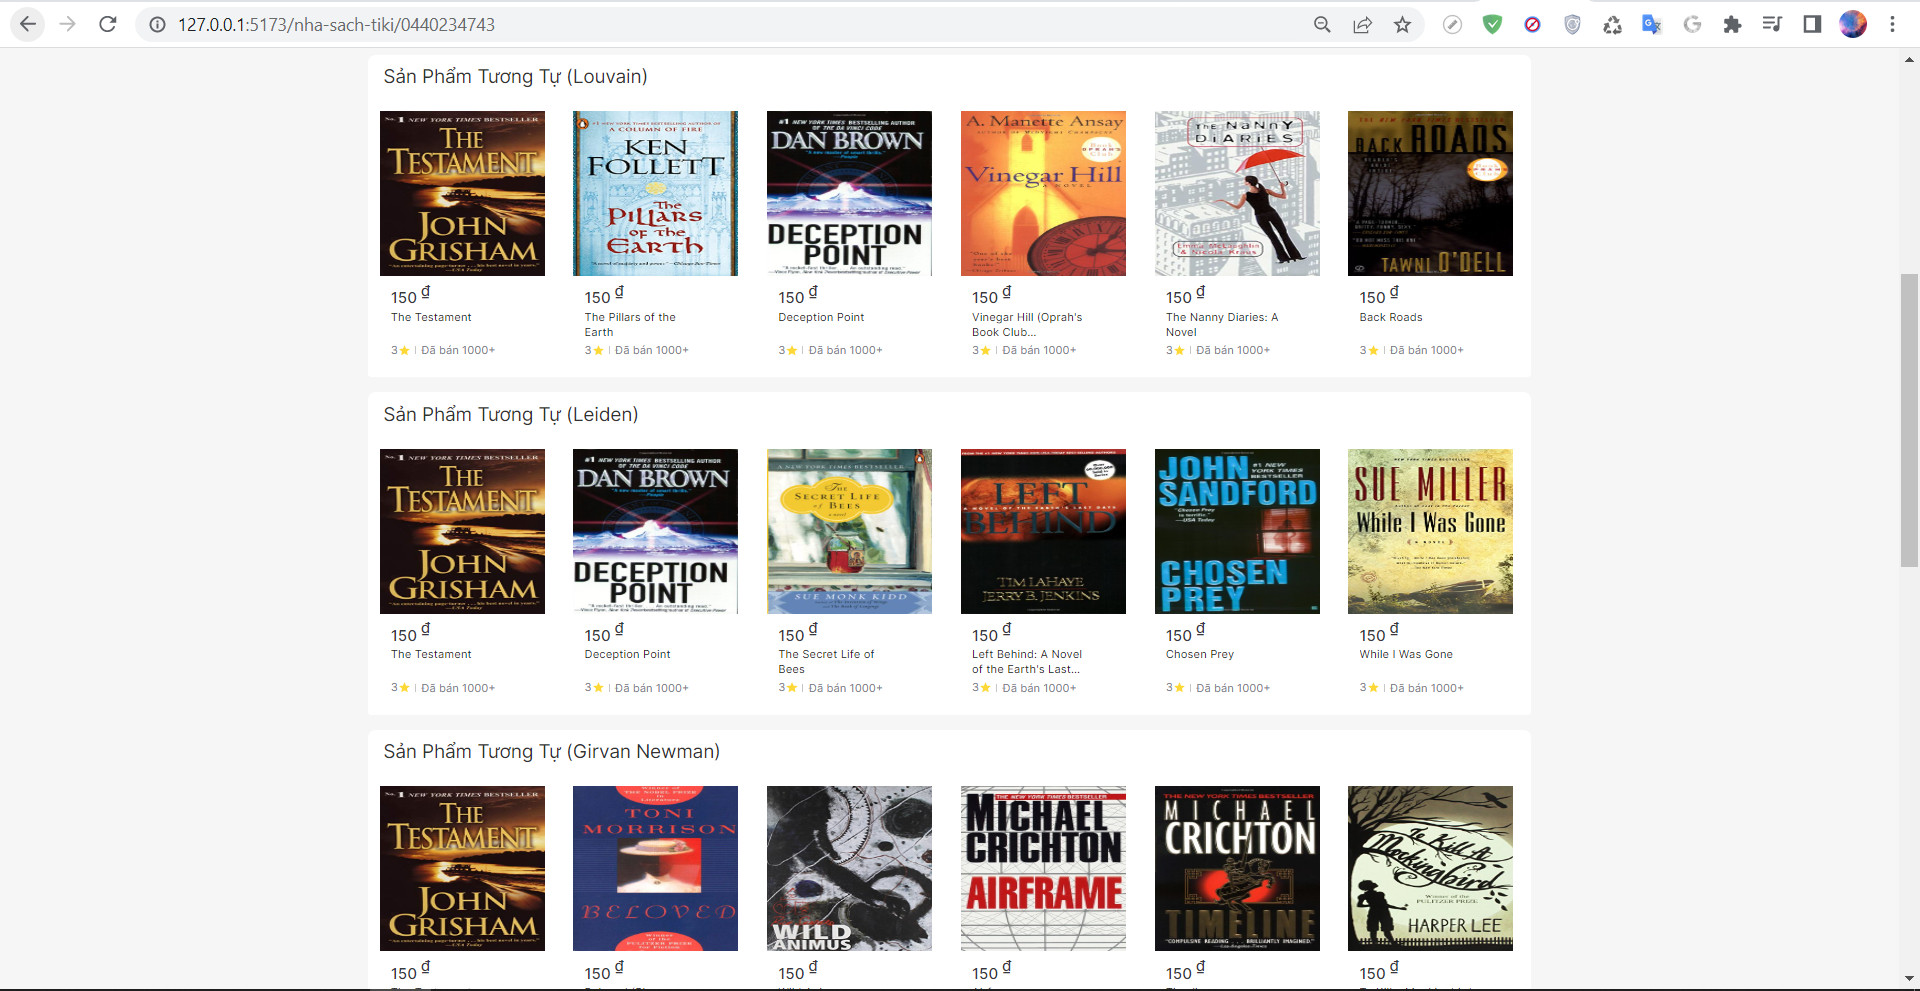
\includegraphics[width=\textwidth]{image/book-detail2.jpg}
            \caption{Book detail page recommendation algorithms}
        \end{figure}
\end{enumerate}

\subsection{Modularity score comparison}
To improve the efficiency of measuring algorithm modularity, we implemented a strategy of dividing the dataset into smaller subsets. Our approach involved selecting the top 500 books that appeared in all book pairs from the previous Map Reduce step. This selection criterion was chosen over random selection from all pairs to avoid generating a sparse graph that would result in significantly lower modularity scores for all three algorithms, making it challenging to measure them accurately.

By ensuring that the selected nodes had the highest number of edges, we aimed to facilitate faster execution of all three algorithms

\begin{figure}[H]
    \centering
    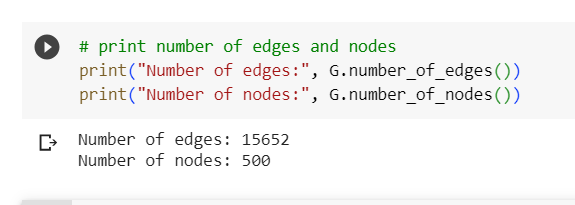
\includegraphics[width=\textwidth]{image/modulairytest.png}
    \caption{Number of edge and node for modularity measurement}
\end{figure}

\begin{figure}[H]
    \centering
    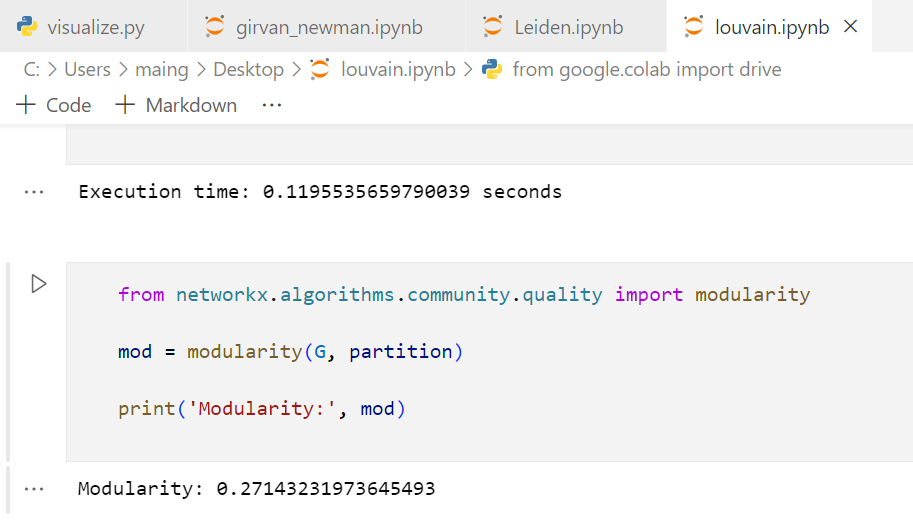
\includegraphics[width=\textwidth]{image/modularity measure louvain.png}
    \caption{modularity measurement for Louvain algorithms}
\end{figure}

\begin{figure}[H]
    \centering
    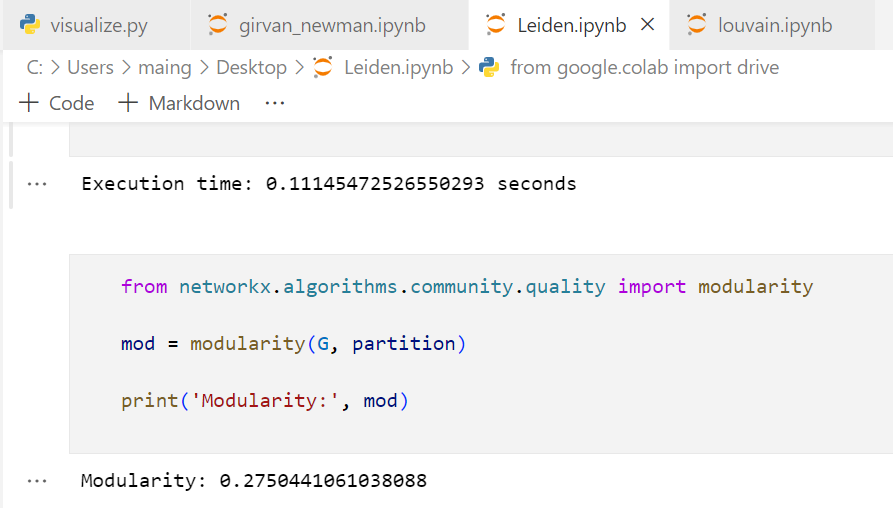
\includegraphics[width=\textwidth]{image/modularity measure leiden.png}
    \caption{modularity measurement for Leiden algorithms}
\end{figure}

\begin{figure}[H]
    \centering
    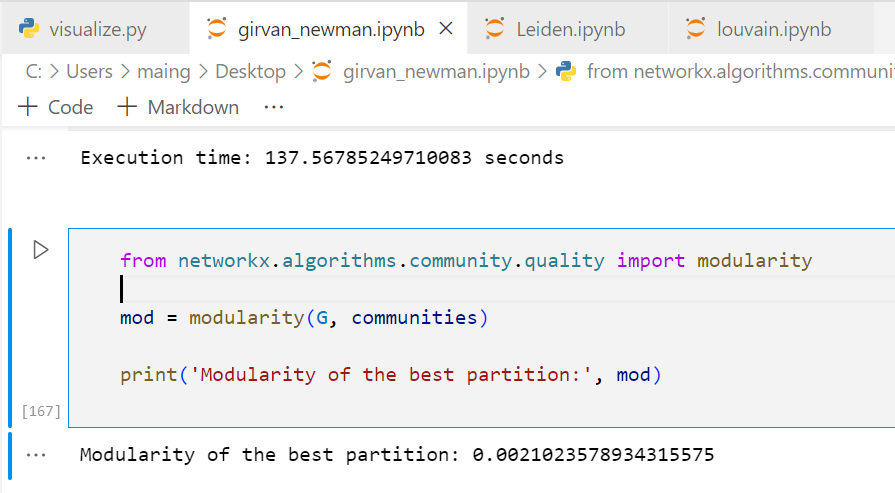
\includegraphics[width=\textwidth]{image/modularity measure girvan.png}
    \caption{modularity measurement for Girvan Newman algorithms}
\end{figure}

Louvain: The Louvain algorithm is recognized for its ability to generate community partitions with high modularity scores. Its iterative optimization process helps identify dense subgraphs and optimize modularity locally and globally.

Leiden: The Leiden algorithm slightly higher score than Louvain.

Girvan-Newman: The Girvan-Newman algorithm tends to have a lower modularity score compared to both Louvain and Leiden. This is because its divisive edge removal approach may not capture the community structure as effectively as the other two algorithms in most cases.

\subsection{Time Efficiency comparison}
To improve the efficiency of measuring algorithm modularity, we implemented a strategy of dividing the dataset into smaller subsets. Our approach involved selecting the top 500 books that appeared in all book pairs from the previous Map Reduce step. To ensured that all three algorithms were executed under similar conditions with large input size.

\begin{figure}[H]
    \centering
    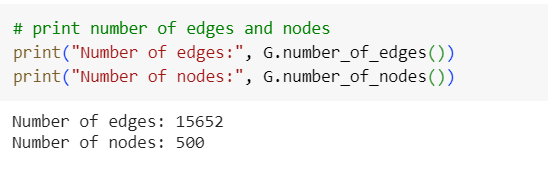
\includegraphics[width=\textwidth]{image/timetest.png}
    \caption{Number of edge and node for time efficiency measurement}
\end{figure}

\begin{figure}[H]
    \centering
    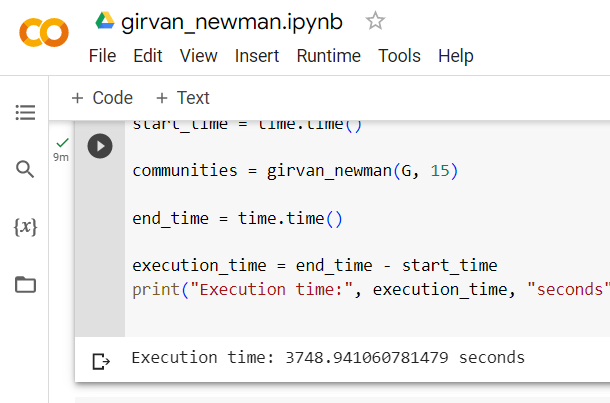
\includegraphics[width=\textwidth]{image/girvantimetest.png}
    \caption{modularity measurement for Girvan Newman algorithms}
\end{figure}

\begin{figure}[H]
    \centering
    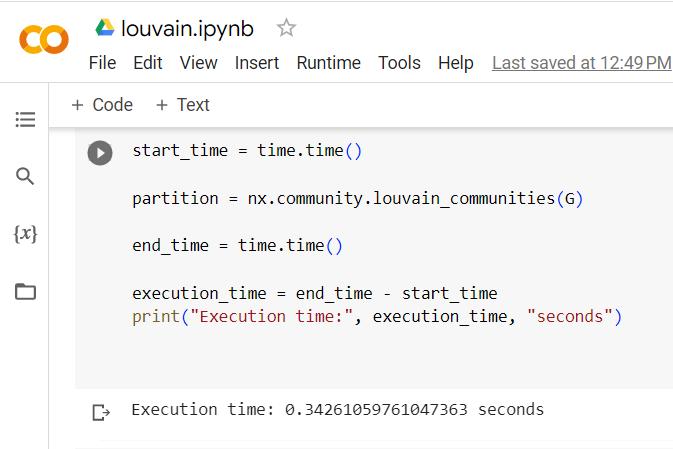
\includegraphics[width=\textwidth]{image/louvaintimetest.png}
    \caption{modularity measurement for Louvain algorithms}
\end{figure}

\begin{figure}[H]
    \centering
    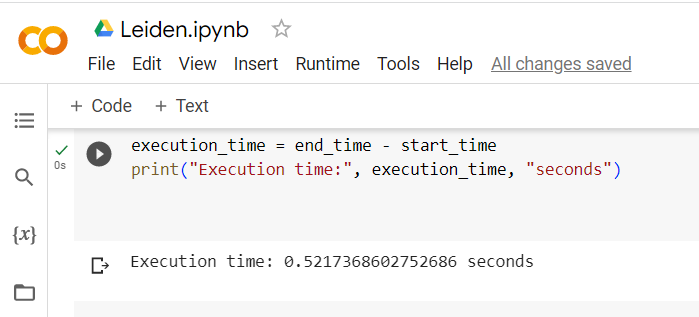
\includegraphics[width=\textwidth]{image/leidentimetest.png}
    \caption{modularity measurement for Leiden algorithms}
\end{figure}

Leiden: The Leiden algorithm is known for its efficiency, particularly in handling large-scale networks. It utilizes techniques such as smart local moving and graph contraction to improve performance.

Louvain: The Louvain algorithm is also efficient and widely used for community detection. It employs a two-phase approach, iteratively optimizing modularity at the local and global levels. However, it can face scalability challenges with very large networks. In this comparison, the execution times of Louvain and Leiden are similar, possibly because the Louvain algorithm has been improved with support from libraries or optimized implementations.

Girvan-Newman: The Girvan-Newman algorithm uses a divisive approach, iteratively removing edges with the highest betweenness centrality to break the graph into communities. This approach is significantly more computationally expensive compared to Louvain and Leiden (3748 seconds), especially for large networks. This is because calculating edge betweenness centrality for all edges can be time-consuming and resource-intensive.

\subsection{Overall comparison}

We have the result of each algorithms: \\

\begin{tabular}{||l|c|c|c||}
    \hline \hline
     & \textbf{Girvan Newman} & \textbf{Louvain} & \textbf{Leiden}  \\ \hline
     \textbf{Modularity} & 0.0021 & 0.2714 & 0.2750\\ \hline 
     \textbf{Time(s)} & 3748.9411 & 0.3426 & 0.5217\\ \hline
     \textbf{Number of} & 12 & 21 & 11\\ 
     \textbf{communities} & & & \\ 
     \hline
     \hline
\end{tabular}
\\
\\
In conclusion, the Louvain and Leiden algorithms generally perform well in terms of modularity score and time efficiency. They are efficient and effective for community detection in various network sizes. However, the Girvan-Newman algorithm, while effective, may not achieve as high modularity scores and much more computationally expensive. It is important to consider the specific characteristics of the network and the desired trade-offs between modularity and runtime when selecting an appropriate algorithm for community detection.
